% modeling/transitions.tex

\chapter{Transition Functions}

% ============================================================
\section*{Motivation}
% ============================================================

Transitions are the decisive element type for curvature-driven alignment
modelling. While fixed elements describe geometric states of constant
curvature, transitions describe the controlled change between such
states.

In railway engineering, transitions are essential for ensuring smooth
vehicle motion, limiting dynamic forces, and satisfying comfort and
safety requirements, as discussed in both engineering-oriented studies
and review literature
\cite{Koc2008TransitionCurves,BrustadDalmo2020Review}.

Within AIM, transitions are not primarily interpreted through explicit
geometric shape, but through the evolution of curvature.

% ============================================================
\section{Definition by Curvature Evolution}
% ============================================================

\begin{principle}[Curvature evolution principle]
Within AIM, transitions are classified primarily by their curvature
evolution rather than by explicit geometric shape.
\end{principle}

\begin{definition}[Transition]
A transition is an alignment element whose curvature varies over its
parameter interval.
\end{definition}

\begin{definition}[Transition curvature law]
Let $L>0$. A transition curvature law is a function
\[
\kappa : [0,L] \to \R
\]
with prescribed boundary values
\[
\kappa(0)=\kappa_0,
\qquad
\kappa(L)=\kappa_1.
\]
\end{definition}

This formulation directly follows the curvature-based description of
planar curves \cite{DoCarmo1976Curves}.

% ============================================================
\section{Normalized Representation}
% ============================================================

\begin{definition}[Normalized transition law]
A normalized transition is defined by
\[
\widehat{\kappa} : [0,1] \to \R
\]
with
\[
\widehat{\kappa}(0)=0,
\qquad
\widehat{\kappa}(1)=1.
\]
\end{definition}

Normalization separates the geometric shape of a transition from its
scale and allows systematic comparison of transition families.

Normalization separates intrinsic transition behaviour from physical
scale and therefore enables reusable transition registries and
family-based modelling.

The following comparison figure answers the engineering question for
transition modelling: when geometric paths appear similar, where do
operationally relevant differences still enter the model?

% ------------------------------------------------------------
% Comparison graphic
% ------------------------------------------------------------

\begin{figure}[ht]
\centering

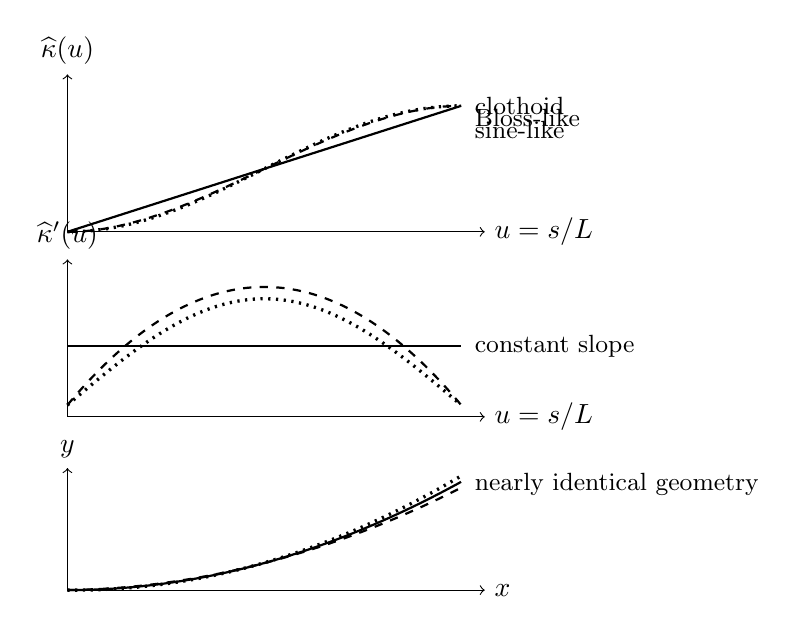
\begin{tikzpicture}[
  scale=1.0,
  axis/.style={->, thin},
  curve/.style={thick},
  label/.style={font=\small}
]

% ------------------------------------------------------------
% Top plot: normalized curvature laws
% ------------------------------------------------------------
\begin{scope}[shift={(0,4.0)}]

  \draw[axis] (0,0) -- (5.3,0)
    node[right] {$u=s/L$};

  \draw[axis] (0,0) -- (0,2.0)
    node[above] {$\widehat{\kappa}(u)$};

  % Clothoid
  \draw[curve]
    plot[smooth, domain=0:5, samples=40]
    (\x,{0.32*\x});

  % Bloss-like
  \draw[curve, dashed]
    plot[smooth, domain=0:5, samples=80]
    (\x,{1.6*(3*(\x/5)^2 - 2*(\x/5)^3)});

  % Sine-like
  \draw[curve, dotted, very thick]
    plot[smooth, domain=0:5, samples=80]
    (\x,{1.6*(0.5 - 0.5*cos(180*\x/5))});

  \node[label,right] at (5.05,1.60) {clothoid};
  \node[label,right] at (5.05,1.45) {Bloss-like};
  \node[label,right] at (5.05,1.30) {sine-like};

\end{scope}

% ------------------------------------------------------------
% Middle plot: derivatives
% ------------------------------------------------------------
\begin{scope}[shift={(0,1.65)}]

  \draw[axis] (0,0) -- (5.3,0)
    node[right] {$u=s/L$};

  \draw[axis] (0,0) -- (0,2.0)
    node[above] {$\widehat{\kappa}'(u)$};

  % Clothoid derivative
  \draw[curve] (0,0.9) -- (5,0.9);

  % Bloss derivative
  \draw[curve, dashed]
    plot[smooth, domain=0:5, samples=80]
    (\x,{0.15 + 1.5*(6*(\x/5)-6*(\x/5)^2)/1.5});

  % Sine derivative
  \draw[curve, dotted, very thick]
    plot[smooth, domain=0:5, samples=80]
    (\x,{0.15 + 1.35*sin(180*\x/5)});

  \node[label,right] at (5.05,0.90) {constant slope};

\end{scope}

% ------------------------------------------------------------
% Bottom plot: geometry
% ------------------------------------------------------------
\begin{scope}[shift={(0,-0.55)}]

  \draw[axis] (0,0) -- (5.3,0)
    node[right] {$x$};

  \draw[axis] (0,0) -- (0,1.55)
    node[above] {$y$};

  \draw[curve]
    plot[smooth, domain=0:5, samples=80]
    (\x,{0.055*\x^2});

  \draw[curve, dashed]
    plot[smooth, domain=0:5, samples=80]
    (\x,{0.052*\x^2 + 0.018*sin(180*\x/5)});

  \draw[curve, dotted, very thick]
    plot[smooth, domain=0:5, samples=80]
    (\x,{0.058*\x^2 - 0.015*sin(180*\x/5)});

  \node[label,right] at (5.05,1.35)
    {nearly identical geometry};

\end{scope}

\end{tikzpicture}

\caption{
Transition families may produce very similar geometric paths while
differing strongly in curvature evolution and curvature derivatives.
This is why transition design must be evaluated in curvature and
dynamic terms, not only in position space.
}
\end{figure}

Transitions that appear nearly identical in position space may differ
substantially in curvature derivatives and therefore in dynamic
behaviour.

The engineering consequence is methodological: transition selection
cannot be justified by geometric fit alone; it must include curvature
evolution and derivative-level runtime criteria.

% ============================================================
\section{Scaling}
% ============================================================

\begin{definition}[Scaled transition law]
\label{def:scaled-transition-law}
Let $L>0$, $\kappa_0,\kappa_1\in\R$, and let $\widehat{\kappa}:[0,1]\to\R$
be a normalized transition law with $\widehat{\kappa}(0)=0$ and
$\widehat{\kappa}(1)=1$. The scaled transition law is
\[
\kappa(s)
=
\kappa_0
+
(\kappa_1-\kappa_0)
\,
\widehat{\kappa}
\!\left(
\frac{s}{L}
\right),
\qquad s\in[0,L].
\]
It satisfies $\kappa(0)=\kappa_0$ and $\kappa(L)=\kappa_1$ by
construction.
\end{definition}

This separates shape from scale and provides the basis for reusable
transition families and parameterized design.

% ============================================================
\section{Regularity and Smoothness}
% ============================================================

\begin{definition}[Regularity class]
A transition is of class $C^k$ if its curvature function is $k$-times
continuously differentiable.
\end{definition}

In engineering practice, higher-order properties such as curvature
derivatives are directly related to ride comfort and dynamic loading,
as shown in both theoretical and engineering studies
\cite{Mieloszyk2012Transition,Koc2017SmoothedEnds}.

\OPEN{Formal role of $\kappa'$ and $\kappa''$ in engineering rules.}

% ============================================================
\section{Transition Families}
% ============================================================

\begin{definition}[Transition family]
A transition family is a class of curvature laws sharing a common
functional structure.
\end{definition}

% ------------------------------------------------------------
\subsection{Classical Families}
% ------------------------------------------------------------

The classical transition curve in railway engineering is the clothoid,
characterized by linear curvature evolution:
\[
\kappa(s)\propto s.
\]

Historically, this line of development can be traced through early work
by Glover \cite{Glover1900TransitionCurves},
Horsburgh \cite{Horsburgh1913TransitionCurve},
and Higgins \cite{Higgins1922TransitionSpiral}.

% ------------------------------------------------------------
\subsection{Polynomial and Alternative Families}
% ------------------------------------------------------------

Polynomial transition curves provide additional flexibility in shaping
curvature evolution and its derivatives.

Such approaches are associated with modern polynomial smoothing research
\cite{ZboinskiWoznica2017Polynomial}
as well as control-oriented constructions proposed by Klauder
\cite{Klauder2001BetterWay,Klauder2009US}.

\TODO{Formal definition of polynomial transition families.}

% ------------------------------------------------------------
\subsection{Geometric Families}
% ------------------------------------------------------------

Some transition curves are introduced through geometric or implicit
relations rather than explicit curvature laws.

\begin{example}
Lemniscate-type or sinusoid-related constructions belong to this class
after suitable reparameterization into curvature space
\cite{Pirti2016Transrapid}.
\end{example}

These curves require transformation into $\kappa(s)$ representation
before they can be integrated into the present framework.

% ------------------------------------------------------------
\subsection{Engineering and Practice-Oriented Families}
% ------------------------------------------------------------

Engineering practice often introduces transition curves through design
rules and operational considerations rather than through purely
theoretical derivation.

The Bloss transition is a notable example of a practical engineering
family, originally described by Bloss \cite{Bloss1978TrackGeometry}
and further discussed in modern summaries \cite{Ciobanu2015Bloss}.

% ------------------------------------------------------------
\subsection{Modern and Hybrid Families}
% ------------------------------------------------------------

Modern engineering practice considers a variety of transition families
with improved dynamic behaviour, smoother endpoint properties, or
higher-order control.

Examples include smoothed-curvature transitions proposed by Koc
\cite{Koc2017SmoothedEnds,Koc2019SmoothedTransition,Koc2019Operational}
and Wiener-Bogen-related approaches
\cite{Wojtczak2017WienerBogen}.

\RESEARCH{Systematic classification of modern transition families.}

% ============================================================
\section{Decomposition Approaches}
% ============================================================

A transition need not always be treated as a single indivisible object.
It may be useful to represent it as a composition of sub-elements.

The Berlinish framework introduced in
\cref{sec:berlinish-composition} provides the concrete decomposition
\[
T=H_{\mathrm{in}}+C+H_{\mathrm{out}},
\qquad
L_{H_{\mathrm{in}}},L_C,L_{H_{\mathrm{out}}}\geq 0.
\]
It is a mathematical composition grammar: zero component lengths and the
choice of half-wave functions determine pure, one-sided, asymmetric, and
compound cases. A sparse implementation may encode the same grammar through a
family identifier, normalized partitions, function references, and parameters.
The mathematical interpretation and its particular data encoding are related,
but not identical.

% ============================================================
\section{Operator View}
% ============================================================

\begin{principle}[Transition operator principle]
A transition element acts as a local curvature evolution operator
transforming one geometric state into another.
\end{principle}

Transitions can therefore be interpreted as state evolution operators
rather than merely as predefined geometric curve shapes.

\RESEARCH{Formal operator algebra of transitions.}

% ============================================================
\section{Implementation Perspective}
% ============================================================

In computational systems, transition curves may be represented using:
\begin{itemize}
\item analytic expressions,
\item polynomial approximations,
\item lookup tables,
\item compiled hybrid representations.
\end{itemize}

Transition families may be represented through registries containing
normalized curvature laws together with derivative and integration
operators.

In the originating system line, \emph{transitionDB} denotes the structured
knowledge base of function identities, half-wave families, parameters, and
known transition forms. The current reference implementation realizes a
substantial part of that role through a validated transition registry: it
contains normalized prototype functions, half-wave descriptors, family
partitions, and named transition entries. This is implementation evidence for
the composition mechanism, not proof that every historical or proprietary
form has been captured.

\emph{TransEd} is the corresponding examination and editing workspace. Its
purpose is to inspect normalized curvature and derivative behaviour and to
work with reusable transition definitions; it does not own Alignment identity
and does not replace alignment-level editing. Analytic expressions and lookup
representations remain alternative realizations of a function law, with the
usual trade-off between traceable exact structure and runtime efficiency.

% ============================================================
\section{Relation to Railway Engineering}
% ============================================================

In railway applications, transitions are tightly coupled to operational
parameters such as speed and cant, and must satisfy strict engineering
constraints
\cite{Kufver2000RailwayAlignment,Klein1998Trassierung}.

The review literature confirms that transition curves must be understood
not only geometrically, but also with respect to comfort, maintenance,
and dynamic response
\cite{BrustadDalmo2020Review}.

% ============================================================
\section{Summary}
% ============================================================

\begin{summary}
Transitions define the controlled evolution of curvature between
geometric states.

Within AIM, they are interpreted as normalized curvature evolution
operators rather than merely as predefined geometric curve types.

Their normalized representation enables reusable transition families,
operator-based modelling, and runtime reconstruction of alignment
geometry and dynamics.
\end{summary}
